\usetikzlibrary{arrows.meta}
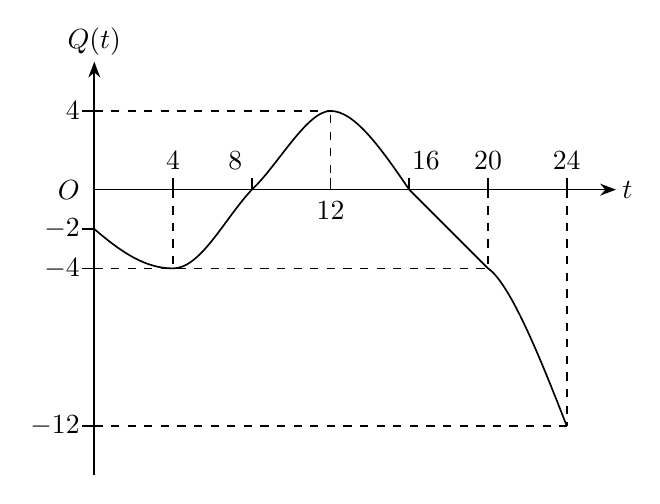
\begin{tikzpicture}[x=0.25cm,y=0.25cm,line width=.6pt,>=Stealth,font=\normalsize]
\coordinate (P0) at (0,-2);
\coordinate (P4) at (4,-4);
\coordinate (P8) at (8,0);
\coordinate (P12) at (12,4);
\coordinate (P16) at (16,0);
\coordinate (P20) at (20,-4);
\coordinate (P24) at (24,-12);
\draw[->] (0,0)--(26.5,0);
\node[right,inner sep=0pt,xshift=2pt] at (26.5,0) {$t$};
\draw[->] (0,-14.5)--(0,6.5);
\node[above,inner sep=0pt,yshift=2pt] at (0,6.5) {$Q(t)$};
\node[left,inner sep=1pt,xshift=-4pt] at (0,0) {$O$};
\draw (4,0)--(4,0.6);
\draw (8,0)--(8,0.6);
\draw (12,0)--(12,0.6);
\draw (16,0)--(16,0.6);
\draw (20,0)--(20,0.6);
\draw (24,0)--(24,0.6);
\draw (0,4)--(-0.6,4);
\draw (0,-2)--(-0.6,-2);
\draw (0,-4)--(-0.6,-4);
\draw (0,-12)--(-0.6,-12);
\node[above,inner sep=0pt,yshift=7pt] at (4,0) {$4$};
\node[above,inner sep=0pt,yshift=7pt,xshift=-6pt] at (8,0) {$8$};
\node[below,inner sep=0pt,yshift=-4pt] at (12,0) {$12$};
\node[above,inner sep=0pt,yshift=7pt,xshift=6pt] at (16,0) {$16$};
\node[above,inner sep=0pt,yshift=7pt] at (20,0) {$20$};
\node[above,inner sep=0pt,yshift=7pt] at (24,0) {$24$};
\node[left,inner sep=1pt,xshift=-4pt] at (0,4) {$4$};
\node[left,inner sep=1pt,xshift=-4pt] at (0,-2) {$-2$};
\node[left,inner sep=1pt,xshift=-4pt] at (0,-4) {$-4$};
\node[left,inner sep=1pt,xshift=-4pt] at (0,-12) {$-12$};
\draw[dashed] (0,4)--(12,4);
\draw[dashed] (0,-4)--(20,-4);
\draw[dashed] (0,-12)--(24,-12);
\draw[dashed] (4,0)--(4,-4);
\draw[dashed] (12,0)--(12,4);
\draw[dashed] (20,0)--(20,-4);
\draw[dashed] (24,0)--(24,-12);
\draw (P0) .. controls (1.4,-3.2) and (2.6,-4) .. (P4)
 .. controls (5.4,-4) and (6.6,-1.5) .. (P8)
 .. controls (9.3,1.2) and (10.8,4) .. (P12)
 .. controls (13.2,4) and (14.5,2.2) .. (P16)--(P20)
 .. controls (21.2,-4.8) and (22.9,-9.2) .. (P24);
\end{tikzpicture}
